%%%%%%%%%%%%%%%%%%%%%%%%%%%%%%%%%%%%%%%%%%%%%
%INTRODUCTION
%%%%%%%%%%%%%%%%%%%%%%%%%%%%%%%%%%%%%%%%%%%%%
% Strcture
%----------
% - Pathogens spread 
% - Distribution of Foc is prime example 
% - TR4 is a strong reason to monitor the distribution and genetic makeup of Fwb pathogens.
% - Lack of data from world's largest producer and climate change is a threat. 
% - We're sequencing isolates...
%%%%%%%%%%%%%%%%%%%%%%%%%%%%%%%%%%%%%%%%%%%%%

\section{Abstract}

\newpage

\section{Introduction}

The history of \acf{Focub} exemplifies the profound impact  pathogen spread and diversification can have on global crop production, economies, and biodiversity. Although first reported in Australia in 1876 by \textcite{Bancroft1876}, current evidence suggests that the centre of origin for \ac{Focub} is Southeast Asia, where it co-evolved with its \textit{Musa} host \parencite{Maryani2019}. The global cultivation of bananas inadvertently facilitated the introduction of \ac{Focub} to new regions, leading to severe damage of banana crops \parencite{Kema2021}.

Notable early dispersion of \ac{Focub1} from it centre of origin occurred in South America. First reports in the region came from Panama and Costa Rica in the 1890s, where \ac{Focub1} acquired the common name, Panama disease \parencite{Ashby1913}. From there, \ac{Focub1} quickly spread across 'Gros Michel' plantations in Jamaica (1903), Suriname (1906), Trinidad and Tobago (1907), Cuba (1908), Guatemala (1910), Colombia (1929), and Venezuela (1930). By the mid 20th century, the banana export industry had been decimated by the \ac{fwb} epidemic. \Ac{Focub1} is now widely distributed in banana producing countries, where it affects many local varieties \parencite{Dita2018}.

Current global production of banana is dominated by the 'Cavendish' variety, which takes its name from William Spencer Cavendish, the sixth duke of Devonshire. 'Cavendish' plants were originally brought to the duke's residence, Chatsworth House, Derbyshire, UK (1829) after their discovery in Southern China in 1826 by British colonial botanists. Shoots from Chatsworth's 'Cavendish' were distributed to British colonies across the globe and resistance to \ac{Focub1} was eventually identified. By the 1950s the banana export industry had substituted the 'Gros Michel' variety for the 'Cavendish' subgroup \parencite{Ploetz2005, Dita2018}. However, in the following decade, 'Cavendish' banana plants in Taiwan were observed displaying symptoms of \ac{Focub} infection \parencite{Agrios2005}. By the 1990s, the same strain of \ac{Focub} was devastating 'Cavendish' plantations in Western Indonesia and peninsular Malaysia \parencite{Kema2021}. Identified in 1994 as \ac{Focub} \ac{tr4} \parencite{Ploetz1994}, the strain affecting 'Cavendish' bananas has continued to spread. \Ac{Focub4} arrived in China from Taiwan in 1996, later expanding to Laos, Myanmar, and Vietnam. A first report was also recorded for Australia in 1997 \parencite{Ploetz2015a}. In 2005, \ac{Focub4} was recorded in the Philippines, rapidly spreading in Mindanao \parencite{Molina2009}. In the past 15 years, first reports of \ac{Focub4} have been published frequently, with occurrences in Pakistan (2012), Lebanon (2013), Oman (2013), Jordan (2013), Mozambique (2013), India (2015), Israel (2016), Colombia (2019), Peru (2021), and Venezuela (2023) (Figure: \ref{fig:FocDis}) \parencite{Butler2013, Ploetz2015a, Ordonez2015, Zheng2018, Thangavelu2019, Garcia-Bastida2020, Maymon2020, Kema2021, Acuna2022,  Herrera2023}.

\begin{figure}[hb!]
  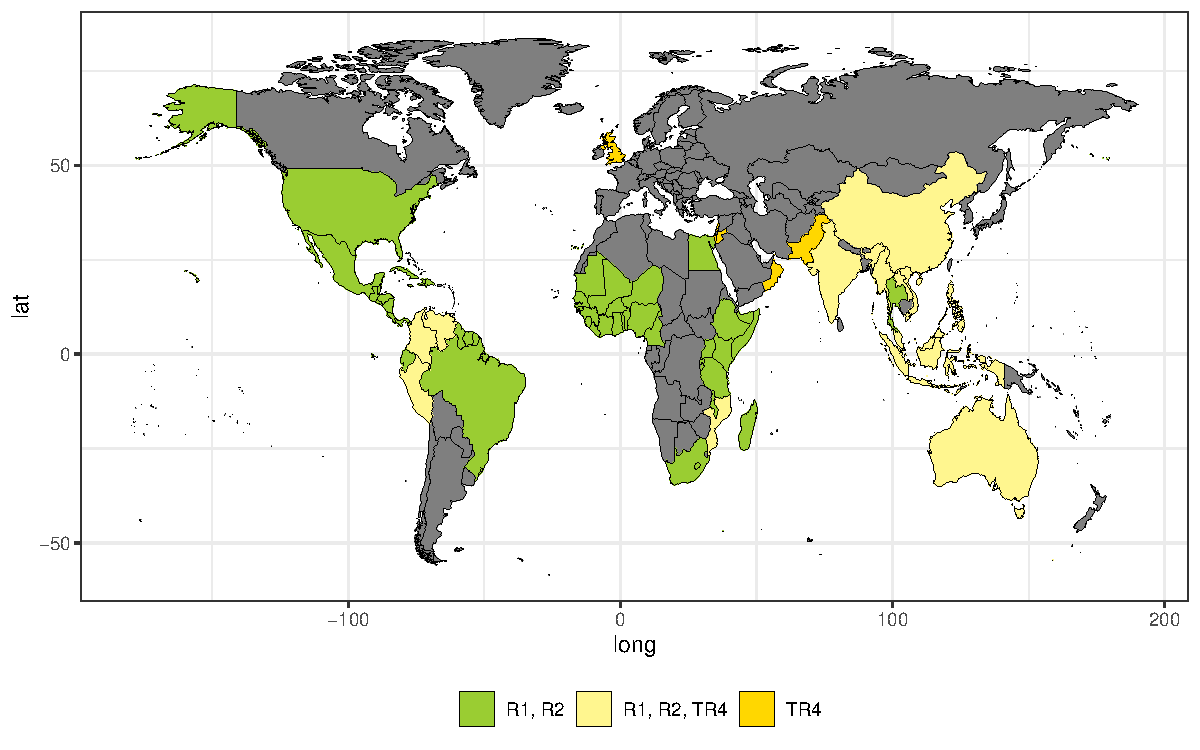
\includegraphics[width=14.5cm]{Figures/FocDis.pdf}
  \caption[Global Distribution of \textit{Fusarium oxysporum} f. sp. \textit{cubense}]{\textbf{Global Distribution of \textit{Fusarium oxysporum} f. sp. \textit{cubense}}. Presence or absence shown by country. Countries which have not reported \ac{Focub} are shown in grey. R1: Race 1, R2: Race 2, TR4: Tropical race 4.}
  \label{fig:FocDis}
\end{figure}

The rapid expansion and evolution of \ac{Focub} poses significant threat to global banana production, particularly in Asia, which serves as the centre of diversity for \ac{Focub}. Accurate monitoring of pathogen distribution and genetic diversity across the region is essential.  Currently, reports of \ac{Focub4} in India, the largest banana-producing country globally, are limited. As the 'Cavendish' cultivar 'Grand Naine' (AAA) accounts for approximately 70\% of India's banana production, \ac{Focub4} is of major concern \parencite{Damodaran2019}. 

In 2017, \ac{r1} and R2 (VCG 0124/5 complex) were the dominant races found in India, with reports in  the southern states of Andhra Pradesh, Karanata, Kerala, and Tamil Nadu, as well, as Gujarat in the east, and Assam, Nagaland, Uttar Pradesh, and West Bengal in the north-west \parencite{Mostert2017, Thangavelu2020}. Concerningly, in 2019, \textcite{Thangavelu2020} reported some \ac{Focub1} isolates (VCGs 0125 and 01220) caused \ac{fwb} symptoms on the 'Cavendish' cultivar 'Grand Naine' (AAA) in Bihar, Uttar Pradesh, Gujarat and Tamil Nadu.  

\Ac{Focub4} was first reported in Barari in the state of Bihar in 2015, and has continued to spread; since  reported in Mansahi, Kursela, Falka, Korha, and Pothia in the Katihar district and in Dhamdhaha and Rupoli in the Purnia district \parencite{Thangavelu2019}. \textcite{Viljoen2020} warned that \ac{Focub4} was likely to spread from Bihar to Madhya Pradesh, Maharashtra, and the Uttar Pradesh, as vehicles and labourers frequently move between the states. \ac{Focub4} has now been reported in Kushi Nagar and Ambedkar Nagar in the state of Uttar Pradesh (Figure: \ref{fig:FocDisIndia}) \parencite{Damodaran2019, Thangavelu2019}, but limited data and no biological materials have been provided to identify the strain(s) present \parencite{Kema2021}. As \ac{Focub} spreads through India, necessitating containment measures, the demand for rapid, precise diagnostics and monitoring of pathogen genetic diversity becomes increasingly evident. Particularly given reports of \ac{Focub1} causing disease in 'Cavendish' varieties \parencite{Thangavelu2020}.

\bigskip
\begin{figure}[h!]
  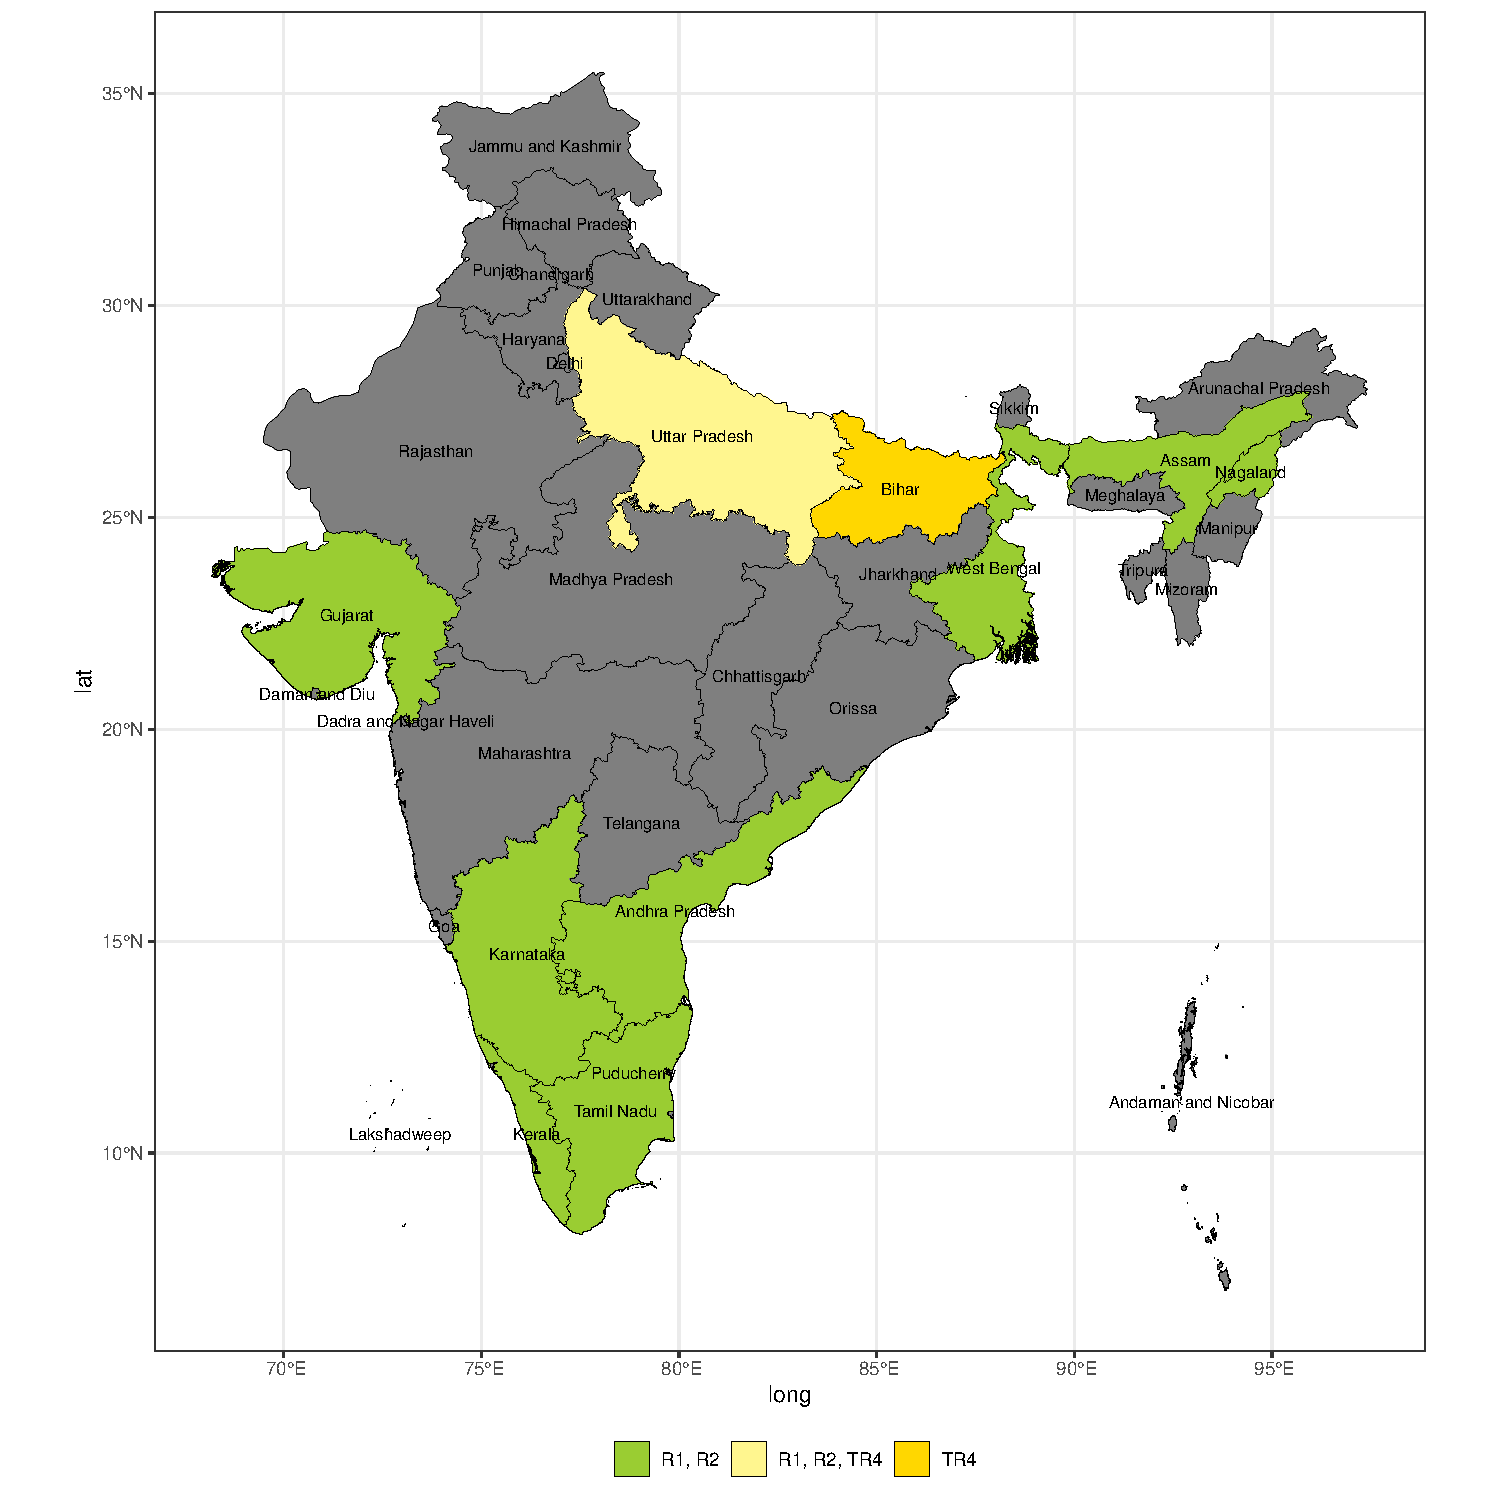
\includegraphics[width=15cm]{Figures/FocDis_India.pdf}
  \caption[Distribution of \textit{Fusarium oxysporum} f. sp. \textit{cubense} in India]{\textbf{ Distribution of \textit{Fusarium oxysporum} f. sp. \textit{cubense} in India}. This map shows presence or absence by region, and does not include subregion. States and Union Territories have been labelled. Regions which have not reported \ac{Focub} are shown in grey. R1: Race 1, R2: Race 2, TR4: Tropical race 4.}
  \label{fig:FocDisIndia}
\end{figure}

Collaborators at \ac{tnau}, India, undertook an assessment of \ac{Focub} diversity in Tamil Nadu. Their primary goal was to explore the genetic and molecular underpinnings of banana resistance against \ac{Focub} using advanced next-generation genomics. A survey was conducted in various banana-growing areas of Tamil Nadu to record symptoms of wilt in different banana cultivars. Samples displaying symptoms of \ac{fwb}, including the \ac{Focub4} susceptible 'Cavendish' banana variety 'Grande Naine', were collected from the field, and the pathogen was isolated and cultured in the laboratory. Among the collected samples, isolates SY-2, S6, S16, and S32 were chosen for further analysis. DNA extraction and PCR amplification were performed to confirm the identity of isolates. The isolated strains, S6, S16, and S32, exhibited severe disease symptoms when inoculated into tissue-cultured 'Grand Naine' banana plants and were classified as highly virulent. PCR amplification using race 4-specific primers\footnote{We have been unable to determine which set of primers were used.} confirmed that SY-2, S6, S16, and S32 were \ac{Focub4} isolates, capable of infecting 'Cavendish' banana (Work conducted at \ac{tnau} is summarised in Appendix \ref{apx:}).

Here, the focus lies on the assembly and analysis of genomic traits within \textit{Fusarium} isolates (SY-2, S6, S16, and S32) retrieved from 'Cavendish' banana plants, an undertaking led by collaborators at \ac{tnau}. Taxonomic identity and genetic diversity are assessed and suggest that there is a potentially novel species of \textit{Fusarium} infecting banana in this region. Of the isolates sequenced, S6 is a \ac{Focub} \ac{r1} isolate, while SY-2, S16, and S32 belong to the \textit{F. fujikuroi} species complex. Phylogenetic analysis, read mapping, and \ac{sixg} profiling supported these classifications. It is important to note, however, that bacterial contamination with \textit{Stenotrophomonas} species was detected in S6 and S32 isolates, warranting future studies to confirm this potentially novel taxon.

%%%%%%%%%%%%%%%%%%%%%%%%%%%%%%%%%%%%%%%%%%%%%
%METHODS
%%%%%%%%%%%%%%%%%%%%%%%%%%%%%%%%%%%%%%%%%%%%%
\newpage

\section{Materials and Methods}

 \subsection{Analysis of Raw Read data from TNAU isolates}

The raw Illumina paired-end reads for the \textit{Fusarium} isolates SY-2, S6, S16, and S32, which are reported to be highly virulent on 'Cavendish' banana, were supplied by collaborators at \ac{tnau}\footnote{\textcolor{red}{Due to communication challenges with collaborators at TNAU, we have not been able to establish the extraction protocol used to produce the DNA used for sequencing.}}. Following FastQC (v0.11.8)
\parencite{Andrews2010} analysis, raw reads were mapped to \ac{Focub4}  isolate UK0001 (\href{https://www.ncbi.nlm.nih.gov/datasets/genome/GCA_007994515.1/}{GCA\_007994515.1}) \parencite{Warmington2019} reference quality genome using BOWTIE2 (v2.4.5) \parencite{Langmead2012} (for full command-line arguments and shells scripts, see: \href{https://github.com/JamiePike/NewTools-Project/blob/master/docs/Assembly/AssemblyNotes.md}{GitHub}) . Due to poor mapping rates for some isolates, 1000 raw reads were extracted from each \ac{tnau} isolate and searched using \ac{ncbi} web-based \acl{blast} (\textcite{Nih2014}). Raw reads from each isolate were also mapped to high-quality assemblies of the \ac{Focub1} isolate 160527 (\href{https://www.ncbi.nlm.nih.gov/datasets/genome/GCA_005930515.1/}{GCA\_005930515.1}) \parencite{Asai2019} and the \textit{Fusairum sacchari} isolate FS66 (\href{https://www.ncbi.nlm.nih.gov/datasets/genome/GCA_017165645.1/}{GCA\_017165645.1}) \parencite{Cui2021}. Isolates S6, S16 and S32 were also mapped to a reference quality \textit{Stenotrophomonas maltophilia} genome assembly, isolate NCTC10258 (\href{https://www.ncbi.nlm.nih.gov/datasets/genome/GCF_900475405.1/}{GCA\_900475405.1}). 

\subsection{Genome Assembly and Annotation}

\subsubsection{\textit{De novo Assembly}}
A \textit{de novo} assembly was generated for each of the \ac{tnau} isolates using SPAdes (v3.14.1) \parencite{Prjibelski2020} following FastQC (v0.11.8) analysis. SPAdes is routinely employed when generating \textit{Fusarium} genomes
(see: \textcite{Armitage2018, Hudson2020, Tanaka2022}). A custom Python script was developed to remove sequences with <25\% GC content from the assembly (see: \href{https://github.com/JamiePike/NewTools-Project/blob/master/bin/gcTrimmer.py}{GitHub}). As raw read data for isolates S6 and S32 contained high levels of contamination, \textit{de novo} assemblies were generated using only reads mapping to reference genomes \ac{Focub1} isolate 160527 (\href{https://www.ncbi.nlm.nih.gov/datasets/genome/GCA_005930515.1/}{GCA\_005930515.1}) \parencite{Asai2019} and \textit{Fusairum sacchari} isolate FS66 (\href{https://www.ncbi.nlm.nih.gov/datasets/genome/GCA_017165645.1/}{GCA\_017165645.1}) \parencite{Cui2021}, respectively. Mapped reads were determined using BOWTIE2 (v2.4.5) and were extracted into separate FASTQ files using Samtools (v1.6, using htslib v1.6) \parencite{Danecek2021}. 

\subsubsection{Contamination Analysis and Quality Assessments}
Blobtools (v1.1.1) \parencite{Laetsch2017} was used for the taxonomic partitioning of the assemblies. The \ac{tnau} assemblies were searched against the \ac{ncbi} nt database using BLASTN and the paired-end raw reads were aligned to each of the assemblies using BOWTIE2 (v2.4.5). Taxonomic hits were ranked at the species level using default BolbTools settings. To extract contigs that were assigned to a non-\textit{Fusarium} genus by BlobTools (v1.1.1), the BlobTools output json file was filtered using blobtools view, with the -r species flag provided. Contigs assigned to a \textit{Fusarium} species or "no-hit" were then extracted and saved in a separate text file. The blobtools seqfilter command with the default settings was then used to extract contigs which were assigned to \textit{Fusarium} or had "no-hit".

The quality and completeness of the assembled, contaminant-filtered genomes was estimated using \ac{busco} with the hypocreales\_odb10 data set \parencite{Manni2021}. The raw reads were mapped back to the assemblies using BOWTIE2 (v2.4.5) and a Qualimap (v2.2.2) assessment was conducted \parencite{Garcia-Alcalde2012}. Quast (v5.0.2) \parencite{Gurevich2013}  and gfastats (v1.3.6) \parencite{Formenti2022} were used to generate assembly quality statistics. 

\subsubsection{Repetitive Element Identification}

Repetitive elements were identified in each contaminant-filtered assembly using RepeatModeler (v2.0.4) \parencite{Flynn2020} including the -LTRStruct option. Once models had been generated, assemblies were masked iteratively with RepeatMasker (v4.1.5) \parencite{Smit2010} using the ouptut from each round used as input for the following masking step. First small, simple repeats were masked using the -noint and -xsmall options; then assemblies were masked using the default RepeatMasker database (Dfam v3.3) \parencite{Storer2021} using the -species Fusarium option; followed by masking using the models generated by RepeatModeler.

\subsubsection{Genome Annotation}
Following masking, the \ac{tnau} genomes were annotated using the MAKER pipeline (v3.01.04) \parencite{Holt2011}, including AUGUSTUS (v3.3) \parencite{Stanke2006} for \textit{ab initio} gene prediction with the “Fusarium” species option. As no RNA sequencing data were available for these isolates, homology evidence from a reference set of 387,728 proteins, from the \ac{ncbi} RefSeq nr database \parencite{Agarwala2016}, generated using the search term "Fusarium AND srcdb\_refseq[PROP]" was used. 

\subsection{Phylogenetic Analysis of \ac{tnau} isolates}\label{chap2:phylogeny}

The common Fusarium genetic barcodes \ac{tef} and \ac{rbp2} were used to generate phylogenies (Edel-Hermann and Lecomte, 2019). A \ac{tef} and \ac{rbp2} sequence database were compiled using available reference sequences from the \ac{ncbi} database (Appendix; \ref{apx:}). Homologs of each barcode were identified in each our database of \ac{Fo} assemblies (See section:~\ref{chap3:fusariumdb}) using BLASTN (v 2.9.0+)(1e-\textsuperscript{6} cut-off). The locations of hits with greater than 70\% identity and 90\% coverage were recorded, and the sequence within this region was extracted using Samtools (v1.15.1). The \ac{tef} and \ac{rbp2} regions from each genome were concatenated into a single FASTA file for each barcode. MAFFT (v7.505) (Katoh \et 2019) was used to construct a multiple sequence alignment adjusting the direction according to the first sequence to ensure correct alignment and any overhanging regions were trimmed manually. IQ-TREE (v2.2.0.3) (Nguyen \et 2015) was used to infer a maximum-likelihood phylogeny using the ultrafast bootstrap setting for 1000 bootstrap replicates and was visualised using iTOL (Letunic and Bork, 2021). 

\subsection{Identification of pathogen-specific features.}

\subsubsection{\textit{Secreted In Xylem} gene searches}

To identify known \acs{Fo} effectors in the \ac{tnau} assemblies and compare the \ac{sixg} profile to other \textit{Fusaria}, reference sequences for SIX1-SIX14 used by \textcite{Czislowski2018} were downloaded from the GenBank and homologs of each \textit{SIX} gene was identified using TBLASTN (v2.9.0+) (1e-6 cut-off) in the \ac{tnau} assemblies, as well as publicly available assemblies of \ac{Focub} (n=14), \textit{F. sacchari} (n=2), the \ac{Fo} endophyte Fo47, \ac{Fo} formae speciales \textit{cepae, conglutinans, coriandrii, lini, lycopersici,  rapae} and \textit{vasinfectum}, and \textit{F. graminearum}, which were downloaded from \href{https://www.ncbi.nlm.nih.gov/data-hub/genome/}{GenBank} following a Genome search. (Supplementary table x: Genomes table). A binary data matrix indicating presence (“1”) or absence (“0”) was generated using the TBLASTN hit data.

\subsubsection{Identification of \acl{mimp} elements}

As \acf{mimp} elements are associated with effectors in \ac{Fo}, \acp{mimp} were identified in the \ac{tnau} isolates, as well as the reference genomes \ac{Focub4} UK0001 (\href{https://www.ncbi.nlm.nih.gov/datasets/genome/GCA_007994515.1/}{GCA\_007994515.1}), \ac{Focub1} 160527 (\href{https://www.ncbi.nlm.nih.gov/datasets/genome/GCA_005930515.1/}{GCA\_005930515.1}) and \textit{Fusairum sacchari} FS66 (\href{https://www.ncbi.nlm.nih.gov/datasets/genome/GCA_017165645.1/}{GCA\_017165645.1}) using a custom python script (see: Appendix ~\ref{apx:mimp_finditer.py}, or \href{https://github.com/JamiePike/NewTools-Project/blob/master/bin/mimp_finditer.py}{GitHub}), which searched for the \ac{mimp} \ac{tir} sequences, "CAGTGGG..GCAA[TA]AA" and "TT[TA]TTGC..CCCACTG". Where sequences matching this pattern occurred within 400 nucleotides of each other a \ac{mimp} was recorded. 

\subsubsection{Identification of putative effectors}

To identify candidate effectors in the \ac{tnau} isolates, the predicted protein set for each isolate was filtered by size (>30aa and <450aa) and submitted to SignalP (v4.1) \parencite{Petersen2011}. Sequences which were predicted to contain a signal peptide were parsed to EffectorP (v2.0.1) \parencite{Sperschneider2018} for effector prediction. The candidate effector sets from each genome were then combined and clustered using CD-HIT (v4.8.1) \textcolor{red}{[NEED TO GET BIB ENTRY FOR (Fu, et al., 2012)]} (\textcolor{red}{percentage identity determined using command line}) to identify candidate effectors profiles. 

\subsubsection{Reference genome alignment and raw read mapping}

Pathogenic chromosomes are common among plant pathogenic \ac{Fo} \parencite{Ma2010, Fokkens2020}. As the \ac{tnau} isolate assemblies were too fragmented to characterise  pathogenic regions, \acp{mimp}, \acp{sixg}, and candidate effectors identified using the Maei pipeline (Chapter \ref{Chap3}) were recorded in the high-quality \ac{Focub4} UK0001 and \textit{F. sacchari} FS66 assemblies, and \ac{tnau} isolate raw reads mapped on to these assemblies using BOWTIE2 (v2.4.5). Nucmer (-max match, deltafilter –g) from MUMmer (v4.0.0rc1) \parencite{Marcais2018} was used to align the ac{Focub4} UK0001 and \textit{F. sacchari} FS66 assemblies to identify shared putative pathogenic regions between the assemblies. Circos (v0.69-8) \parencite{Krzywinski2009} was used to visualise virulence factor location and genome alignments. 

\subsection{Data and software availability}

The full pipelines, command-line arguments as well as bash, R, and python scripts for all analysis outlined above are available on \href{https://github.com/JamiePike/NewTools-Project}{GitHub}, with supporting documentation provided in Markdown format.

%%%%%%%%%%%%%%%%%%%%%%%%%%%%%%%%%%%%%%%%%%%%%
%RESULTS
%%%%%%%%%%%%%%%%%%%%%%%%%%%%%%%%%%%%%%%%%%%%%
\newpage

\section{Results}
\subsection{Summary of phenotyping and genotyping data supplied by TNUA}

The collaborative study was undertaken by researchers at \acs{tnau} and aimed to investigate the diversity of \ac{Focub} in Tamil Nadu and explore the mechanisms of resistance against this pathogen in banana using advanced genomics techniques. The initial step involved a comprehensive survey conducted across various regions in Tamil Nadu to document and assess wilt symptoms in different banana cultivars.

Samples exhibiting symptoms of \textit{Fusarium} wilt, including the widely grown 'Grande Naine' Cavendish banana variety susceptible to \acs{Focub4}, were collected. The isolated pathogen was successfully cultured under controlled laboratory conditions and Koch's postulates confirmed. Confirmatory tests based on DNA extraction and PCR amplification were carried out to validate the identity of the isolates. Intriguingly,  isolates S6, S16, and S32 displayed a robust ability to induce severe disease symptoms upon inoculation into tissue-cultured 'Grand Naine' banana plants, and were classified as highly virulent.

Further investigations using race 4-specific primers in PCR amplification confirmed that the isolated S6, S16, and S32 strains belonged to the \acs{Focub4} group, demonstrating their capacity to infect Cavendish banana. As a consequential step, the isolates underwent sequencing. However, specific details such as the sequencing platform and statistical insights derived from the sequencing data remain pending due to ongoing communication challenges with \ac{tnau} collaborators.

\subsection{Analysis of Raw Read data from TNAU isolates}

Raw read mapping of the S6, S16, S32, and SY-2 to the \ac{Focub4} UK0001 assembly produced an 8.72\%, 53.81\%, 15.69\%, and an 54.11\% alignment for all raw reads, respectively (Table ~\ref{tab:RawReadMapping}). Due to the low alignment rates, unmapped reads were extracted and a random subset of 1000 reads per isolate was searched using \acf{ncbi} web BLASTn \parencite{Nih2014}. For isolates S6 and S32, the majority of hits with >90\% coverage and identity were for \textit{Stenotrophomonas} species, particularly \textit{Stenotrophomonas maltophilia}. Further, the raw S6 and S32 reads show a similar GC\% to the \textit{S. maltophilia }reference genome assembly (\href{https://www.ncbi.nlm.nih.gov/datasets/genome/GCF_900475405.1/}{GCA\_900475405.1}) (S6=63\% GC content, S32=61\% GC content, \textit{S. maltophilia} reference=66.5\% GC content). For isolate S16, the majority of hits for unmapped reads with >90\% coverage and identity against the NCBI database were for \textit{Fusarium fujikuroi}. 

\bigskip
% Please add the following required packages to your document preamble:
% \usepackage{booktabs}
% \usepackage{multirow}
% \usepackage{graphicx}
\begin{table}[h!]
\caption[Overall alignment rate of all raw reads from each TNAU isolates to fungal and bacterial reference species]{{\textbf{Overall alignment rate of all raw reads from each TNAU isolates to fungal and bacterial reference species.}} Overall alignment rate determined by Bowtie2 (version 2.4.5). Reference assemblies were downloaded from GenBank: \ac{Focub4} isolate UK0001 (\href{https://www.ncbi.nlm.nih.gov/datasets/genome/GCA_007994515.1/}{GCA\_007994515.1}), \ac{Focub1} isolate 160527 (\href{https://www.ncbi.nlm.nih.gov/datasets/genome/GCA_005930515.1/}{GCA\_005930515.1}), \textit{Fusairum sacchari} isolate FS66 (\href{https://www.ncbi.nlm.nih.gov/datasets/genome/GCA_017165645.1/}{GCA\_017165645.1}), \textit{Stenotrophomonas maltophilia} isolate NCTC10258 (\href{https://www.ncbi.nlm.nih.gov/datasets/genome/GCF_900475405.1/}{GCA\_900475405.1}).}
\label{tab:RawReadMapping}
\centering
\resizebox{\textwidth}{!}{%
\begin{tabular}{cccccc}
\hline
\multirow{2}{*}{\textbf{Reference Species}} & \multirow{2}{*}{\textbf{Strain}} & \multicolumn{4}{c}{\textbf{BOWTIE2 Alignment Rate}} \\ \cline{3-6} 
 &  & \textbf{S6} & \textbf{S16} & \textbf{S32} & \textbf{SY-2} \\ \cline{1-2}
\textit{Fo.} f. sp. \textit{cubense} (TR4) & UK0001 & 8.72\% & 53.81\% & 15.69\% & 54.11\% \\
\textit{Fo.} f. sp. \textit{cubense} (R1) & 160527 & 9.90\% & 53.67\% & 15.51\% & 54.02\% \\
\textit{F. sacchari} & FS66 & 5.24\% & 68.65\% & 22.49\% & 93.96\% \\
\textit{Stenotrophomonas maltophilia} & NCTC10258 & 49.32\% & 0.01\% & 53.93\% & -- \\ \hline
\end{tabular}%
}
\end{table}
\bigskip

Isolates S6, S16 and S32 were also mapped to a reference quality \textit{Stenotrophomonas maltophilia} genome due to the high number of BLAST hits. Approximately 50\% of raw reads from isolates S6 and S32 mapped to the \textit{S. maltophilia} reference, whereas raw reads from isolate S16 only had a 0.01\% mapping rate to the \textit{S. maltophilia} reference (Table ~\ref{tab:RawReadMapping}) Raw reads from isolates S6 and S32 had a 5.24\% and 22.49\% mapping rate to the \textit{F. sacchari} reference, respectively, whereas 68.65\% of the raw reads from isolate S16 and 93.96\% of the raw reads from the SY-2 isolate mapped to the \textit{F. sacchari} reference.

\subsection{\textit{De novo} Genome Assembly and Contamination Analysis}

As raw read alignment rates for the \ac{Focub1} (\href{https://www.ncbi.nlm.nih.gov/datasets/genome/GCA_005930515.1/}{GCA\_005930515.1}) and \ac{Focub4} (\href{https://www.ncbi.nlm.nih.gov/datasets/genome/GCA_007994515.1/}{GCA\_007994515.1}) reference assemblies were <55\% for all \ac{tnau} isolates, a \textit{de novo} approach using SPAdes (v3.14.1) was used for genome assembly. Following assembly, contigs with \textless 25\% GC content were removed from the SY-2 and S16 assemblies, reducing the total number of contigs from XX to XX in the SY-2 assembly and 1666 to 768 in the S16 assembly. The contaminant filtered S6 \textit{de novo} assembly generated using the \ac{Focub1} 160527 (\href{https://www.ncbi.nlm.nih.gov/datasets/genome/GCA_005930515.1/}{GCA\_005930515.1}) mapped reads contained 6048 contigs, and the contaminant filtered S32 \textit{Fusairum sacchari} FS66 (\href{https://www.ncbi.nlm.nih.gov/datasets/genome/GCA_017165645.1/}{GCA\_017165645.1}) mapped reads contained 2443 contigs. 

The SY-2 S6, S16, and S32 assemblies recorded 99.6\%, 97.5\%, 97.4\%, and 97.4\% \ac{busco} intact, single copies orthologs (hypocreales\_odb10 dataset), respectively. Coverage ranged from 16x for the S6 assembly to 148x for the S16 assembly (Table~\ref{tab:TNAUAssemblyStats}).

\bigskip
% Please add the following required packages to your document preamble:
% \usepackage{multirow}
% \usepackage{longtable}
% Note: It may be necessary to compile the document several times to get a multi-page table to line up properly
\begingroup
\setlength{\tabcolsep}{20pt} % Default value: 6pt
\renewcommand{\arraystretch}{0.9}
\setlength\LTcapwidth{\textwidth} % default: 4in (rather less than \textwidth...)
\setlength\LTleft{0pt}            % default: \parindent
\setlength\LTright{0pt}           % default: \fill
\begin{longtable}[c]{ccccc}
\caption[Summary statistics of TNAU genome assemblies.]{\textbf{Summary statistics of TNAU genome assemblies. }\textit{De novo} assemblies generated using SPAdes (version 3.14.1) with all raw reads supplied by Tamil Nadu Agricultural University. }
\label{tab:TNAUAssemblyStats}\\
\hline
\multirow{\textbf{\begin{tabular}[c]{@{}l@{}}Assembly\\Statistic\end{tabular}}} & \multicolumn{4}{c}{\textbf{TNAU Isolate Assembly}} \\ \cline{2-5} 
                    & \textbf{SY-2}    & \textbf{S6} & \textbf{S16} & \textbf{S32} \\ \hline
\endfirsthead
%
\multicolumn{5}{c}%
{{\bfseries Table \thetable\ continued from previous page}} \\
\endhead
%
Number of contigs   & 441      &                & 768       & 2443        \\
Largest contig (Mb) & 0.87     &                & 0.88      & 0.77        \\
Total length (Mb)   & 44.35    &                & 44.86     & 40.92       \\
GC (\%)             & 47.97    &                & 47.53     & 48.85       \\
N50 (bp)            & 221769   &                & 234991    & 78523       \\
L50                 & 57       &                & 60        & 109         \\
Mapped Reads (\%)   & 99.6     &                & 99.53     &             \\
Mean Coverage       & 73x      &                & 148x      &             \\ 
BUSCO (\%)          & 99.6     &                & 97.4      & 97.4        \\\hline  


\end{longtable}
\endgroup
\bigskip

Although the S6 and S32 isolates had high mapping rates to the \textit{S. maltophilia} reference, unfiltered raw read data were used to generate a \textit{de novo} assembly to assess for taxonomic partitioning using BlobTools (v1.1.1) (Laetsch and Blaxter, 2017). The S6 and S32 unfiltered and unmapped assemblies generated using all raw reads contained 100,147 and 1,048 contigs, had a BUSCO completeness score of 97.7\% and 97.7\%, were 97.64Mb and 49.62Mb in length and had a GC\% of 46.75 and 49.80, respectively. The S6 assembly generated using all raw reads was much larger than is typical for a \ac{Fo} assembly and was highly fragmented. 

\subsubsection{BlobTools analysis reveals contamination in the S6 and S32 raw read data}

The Blobtools analysis showed \textit{Fusarium fujikuroi} accounted for the majority of the \ac{ncbi} nt database TaxID hits for each contig for the S16 isolate and SY-2 assemblies, with 453 and \textcolor{red}{[HOW MANY?]} contigs assigned to this species, respectively (Figures). 

\captionsetup{subrefformat=parens}

\begin{figure}[hp!]
    \centering
    \begin{subfigure}[]{0.9\textwidth}
        \centering
        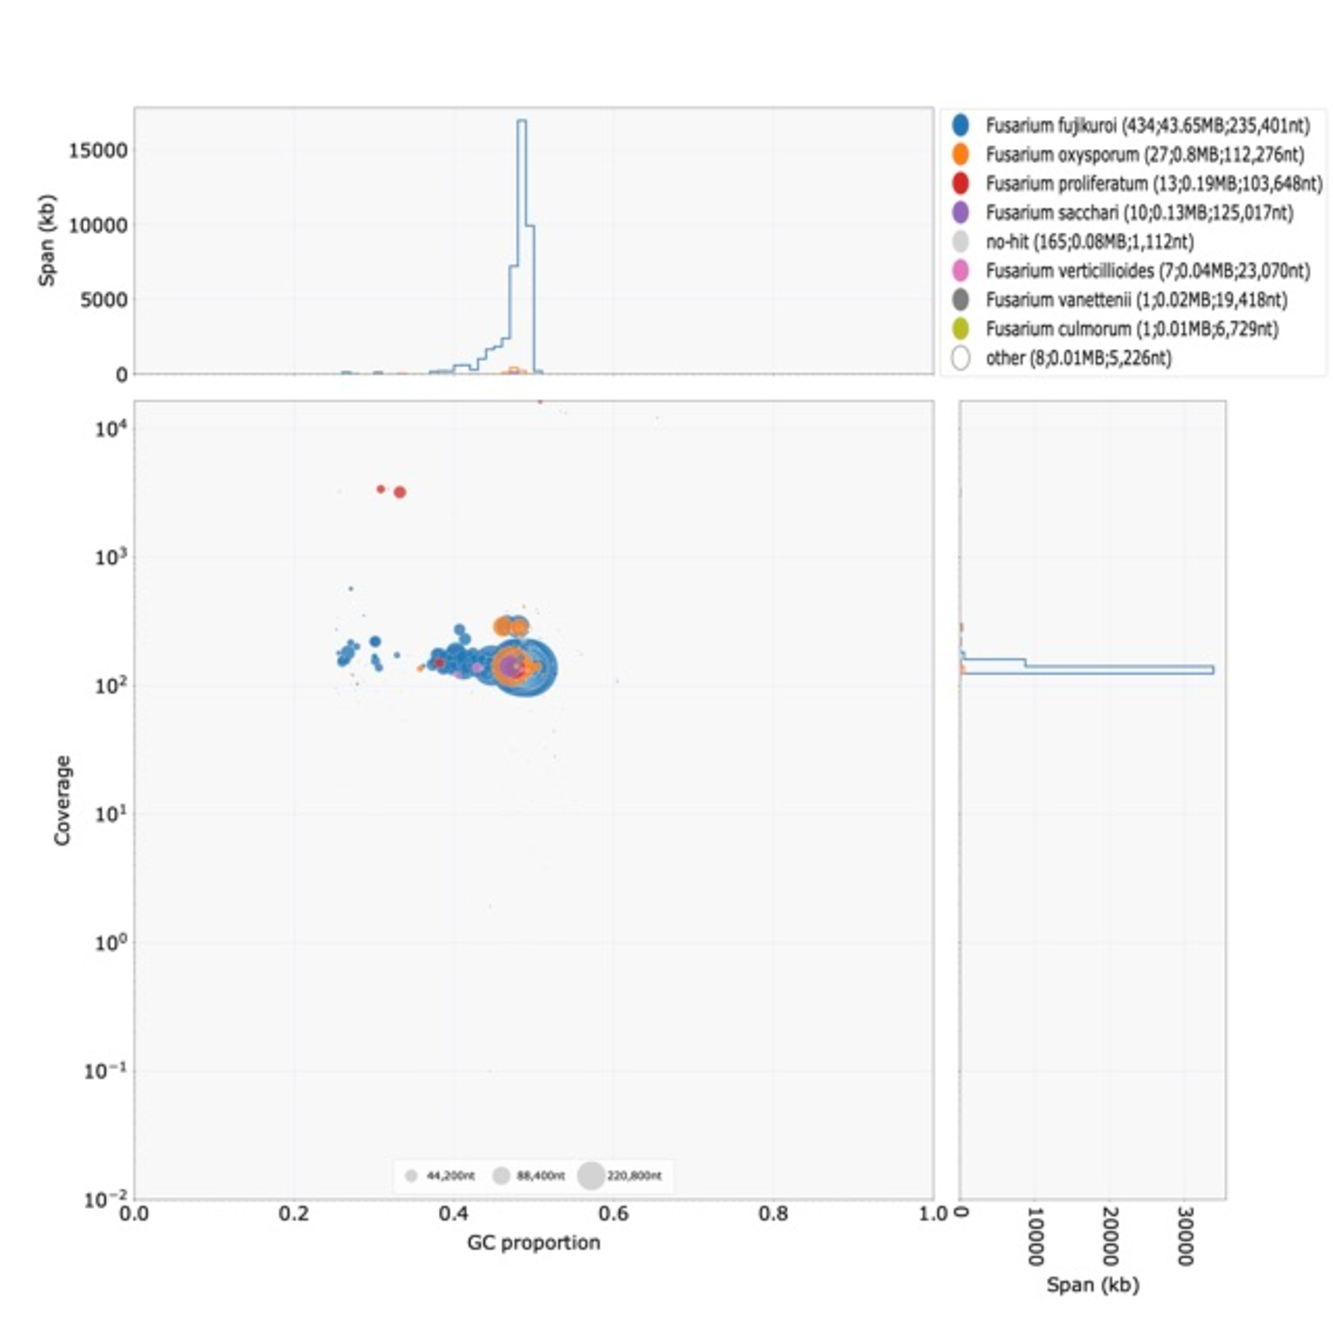
\includegraphics[width=\textwidth]{Figures/TNAU_S16.species.blobplot.pdf}
        \caption{}
        \label{fig:BlobPlot-S16}
    \end{subfigure}
    \begin{subfigure}[]{0.9\textwidth}
        \centering
        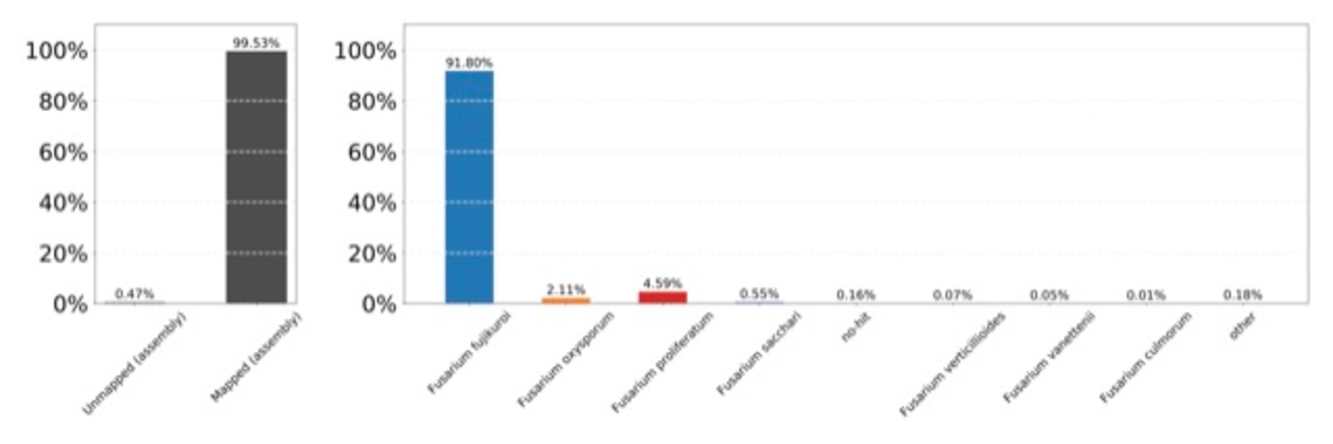
\includegraphics[width=\textwidth]{Figures/TNAU_S16.blobtools.blobDB.json.bestsum.species.p8.span.100.blobplot.read_cov.bam0.pdf}
        \caption{}
        \label{fig:BlobPlot_readcov-S16}
    \end{subfigure}
    \caption[BlobTools visualisations of the S16 assembly]{\textbf{BlobTools visualisations of the S16 assembly shows \textit{Fusarium fujikuroi} is the most common species hit.}
        \subref{fig:BlobPlot-S16} BlobPlot of S16. Sequences in the assembly are depicted as circles, with diameter proportional to sequence length and coloured by taxonomic annotation based on BLASTN (v2.9.0+) of NCBI nt database.
        \subref{fig:BlobPlot_readcov-S16} Read coverage plot of the S16 assembly. Mapped reads are shown by taxonomic group at the rank of species.}
\end{figure}
\bigskip


The \textit{de novo} assemblies generated using all raw reads for the S6 and S32 isolates contained a large number of contigs that had either no hits or were assigned to other genera. For instance, the majority of contigs for the \textit{de novo} S6 assembly had no hits (Figure 2). Some of the contigs had \textit{F. fujikuroi} and \ac{Fo} assigned. The remaining contigs had the greatest sequence similarity to bacterial species. The majority of contigs from the S32 \textit{de novo} assembly had the greatest sequence similarity to \textit{Fusarium} species, particularly \textit{F. fujikuroi}, although some contigs were assigned to \textit{Stenotrophomonas} species, as was observed in the BLAST search of unmapped raw reads (Figure 3). 

The \textit{de novo} assemblies generated for S6 and S32 using reads that mapped to the \ac{Focub1} or \textit{F. sacchari} references were also assessed for taxonomic partitioning using BlobTools. The S6 \textit{de novo} assembly built using \ac{Focub1} mapped reads contained hits from \textit{Fusarium} species, including \textit{F. fujikuroi} and \ac{Fo}, no other genera were assigned to any contigs in this assembly, although \textcolor{red}{2,263} contigs had no hits (Figure 6).  Similarly, the S32 \textit{de novo} assembly was built using \textit{F. sacchari} mapped reads contained hits from \textit{Fusarium} species and no other genera were assigned to any contigs in this assembly (Figure 7). 
 
\subsection{Results from \acf{tef} and \acf{rbp2} phylogeny and database searches showing novel clade}

The common Fusarium genetic barcode (Edel-Hermann and Lecomte, C., 2019) was used for phylogenetic analysis of the TNAU isolates alongside other Fusarium species. The SY-2 isolate \ac{tef} sequence extracted for the phylogeny shared in June 2022 was also included in this phylogeny for reference. For the S16 isolate, the \ac{tef} sequence was extracted from the GC-trimmed de novo assembly. For the S6 and S32 isolates, the \ac{tef} sequence was extracted from the de novo assemblies generated using all raw reads as well as the de novo assemblies generated using the reference mapped reads. 

Using a \ac{tef} database compiled from available reference sequences on the NCBI database, homologs of the \ac{tef} barcode were identified in each TNAU isolate assembly through BLASTN (1e-6 cut-off). For each assembly, the locations of hits with greater than 70\% identity and 90\% coverage were recorded, and the sequence within this region was extracted using Samtools (v1.15.1). Using the extracted \ac{tef} sequences the Fusariod-ID MSLT database and NCBI BLAST database were searched for similar sequences. For the S16 isolate, the Fusariod MSLT database's best scoring hits were for \ac{FFSC}, in which \textit{F. sacchari} can be found (Tables: \ref{tab:Tef1-MLSTdb} \ref{tab:Tef1-NCBIdb}). Further, a search of the \ac{ncbi} database revealed that the \ac{tef} sequence extracted from the S16 assembly's best scoring hits were for \textit{F. sacchari}. Searches for the S6 isolate extracted \ac{tef} sequences suggest this isolate belongs to the \ac{FOSC}. Although there were matches for \ac{Focub} \ac{tef} sequences, these were not in the top 3 results from searches of both databases for the S6 isolate. This may be due to the quality of the S6 assembly. No matches were found for the S32 extracted \ac{tef} sequences in the Fusarioid-ID MSLT database, and hits against the \ac{ncbi} GenBank database were for \textit{F. fujikuroi} isolates. 

% % Please add the following required packages to your document preamble:
% \usepackage{multirow}
% \usepackage{graphicx}
% \usepackage{lscape}
\begin{landscape}
\begin{table}[]
\centering
\captionsetup{width=\linewidth} 
\caption{[\Ac{tnau}\acf{tef} \acf{ncbi} and Fusariod-ID MSLT database searches.]\textbf{Best hits of extracted \acf{tef} sequences from the \acf{tnau} isolate \textit{de novo} assemblies against the Fusariod-ID MSLT database and \ac{ncbi}}}
\label{tab:Tef1-MLSTdb}
\resizebox{\columnwidth}{!}{%
\begin{tabular}{cccc}
\multirow{2}{*}{\textbf{TNAU Isolate Assembly}} & \multicolumn{3}{c}{\textbf{Fusariod-ID MSLT database}}                                     \\ \cline{2-4} 
                                                & Match 1                      & Match 2                      & Match 3                      \\ \hline
\textbf{S6 All reads}                           & \textit{F. oxysporum} Species Complex & \textit{F. oxysporum} Species Complex & \textit{F. oxysporum} Species Complex \\
\textbf{S6 \textit{F. oxysporum}  Reads}                 & \textit{F. oxysporum} Species Complex & \textit{F. oxysporum} Species Complex & \textit{F. oxysporum} Species Complex \\
\textbf{S16}                                    & \textit{F. oxysporum} Species Complex  & \textit{F. oxysporum} Species Complex  & \textit{F. oxysporum} Species Complex  \\
\textbf{S32 All reads}                          & No Matches                   & No Matches                   & No Matches                   \\
\textbf{S32 \textit{F. oxysporum}  Reads}                & No Matches                   & No Matches                   & No Matches                   \\
\textbf{S32 \textit{F. oxysporum}}                        & No Matches                   & No Matches                   & No Matches                  
\end{tabular}%
}
\end{table}
\end{landscape} % Put in appendix, you can state this in the text. 
\bigskip
% Please add the following required packages to your document preamble:
% \usepackage{multirow}
% \usepackage{graphicx}
% \usepackage{lscape}
\begin{table}[h!]
\centering
\captionsetup{width=\linewidth} 
\caption[\Ac{tnau}\acf{tef} \acf{ncbi} and Fusariod-ID MSLT database searches.]{\textbf{Best hits of extracted \acf{tef} sequences from the \acf{tnau} isolate \textit{de novo} assemblies using \ac{ncbi} web-BLASTN.}}
\label{tab:Tef1-NCBIdb}
\resizebox{\columnwidth}{!}{%
\begin{tabular}{cccc}
\multicolumn{1}{l}{\multirow{2}{*}{\textbf{TNAU Isolate Assembly}}} & \multicolumn{3}{c}{\textbf{NCBI database}}                                        \\ \cline{2-4} 
\multicolumn{1}{l}{}                                       & Hit 1                    & Hit 2                    & Hit 3                       \\ \hline
\textbf{S6}                            & \textit{F. o.} isolate 170 & \textit{F. o.} f. sp. \textit{koae} & \textit{F. o.} f. sp. \textit{dianthi} \\
\textbf{S16}                                               & \textit{F. sacchari} CBS:147.25   & \textit{F. sacchari} NRLL 66326  & \textit{F. globosum} CBS:428.97      \\
\textbf{S32}                             & \textit{F. fujikuroi} I1.3        & \textit{F. fujikuroi} IMI 58289   & \textit{F. fujikuroi} Augusto2 \\ 
\textbf{SY-2} & \textit{F. fujikuroi} I1.3        & \textit{F. fujikuroi} IMI 58289   & \textit{F. fujikuroi} Augusto2 \\ \hline     
\end{tabular}%
}
\end{table}
\bigskip

The \ac{tef} regions from each \ac{tnau} assembly and the in-house \ac{tef} database were also used to build a phylogenetic tree. \Ac{tef} sequences were extracted from the \ac{tnau} isolates and aligned to \ac{tef} sequences from other \textit{Fusarium} species as we as \ac{Fo} \ac{fsp}. IQ-TREE (v2.2.0.3) was used to infer a maximum-likelihood phylogeny using the ultrafast bootstrap setting for 1000 bootstrap replicates (Nguyen 2015). The \ac{tef} phylogeny revealed that the  S16 isolate sits within the same clade as the SY-2 isolate and reference \textit{F. sacchari} species which, taken together with the BOWTIE2 raw read mapping data, suggests these isolates may be strains of \textit{F. sacchari} pathogenic towards banana (Figure: ~\ref{fig:TEF1aPhylo}). 

The S32 isolate appears to be a sister lineage of \textit{F. sacchari}, instead, S32 grouping with the novel \textit{Fusarium} species of, \textit{F. mindanaoense}, recently reported in the Philippines by Nozawa, \et (2023) infecting Cavendish banana. The authors suggest that \textit{F. mindanaoense} is a member of the \ac{FFSC} and has acquired the \ac{sixg} \textit{SIX6}, though they have not confirmed the \textit{SIX6} homolog identified is involved in virulence in their novel species.

The S6 isolate clusters within one the \ac{Focub} clades which, alongside the higher mapping rate for to the \ac{Focub} reference and Fusariod-DB and \ac{ncbi} BLASTN results, suggests S6 is a \ac{Focub} isolate. Interestingly, based on the \ac{tef} phylogeny, S6 clusters within a \ac{Focub1} clade, but collaborators at \ac{tnau} suggest that S6 is highly virulent against Cavendish banana varieties. Due to the high amounts of contamination in the S6 raw data, it is challenging to determine the phylogenetic origin of the S6 isolate. Virulence assays comparing S6 to a \ac{r1} reference with high-quality genome sequence available, such as \ac{Focub1} strain 160527 published by Asai., \et (2019), to identify changes associated with enhanced virulence.

\bigskip
\begin{figure}[htp!]
    \centering
    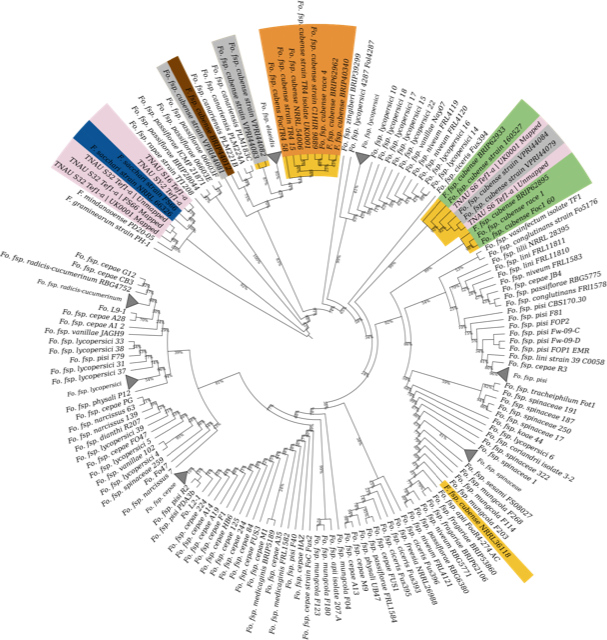
\includegraphics[width=14cm]{Figures/TEF1aPhylo-Including_mindanoense.png}
    \caption[\Acl{tef} phylogeny of \acl{tnau} \textit{Fusarium} isolates.]{\textbf{\Acl{tef} phylogeny of \acl{tnau} \textit{Fusarium} isolates.} \Ac{tnau} isolates S16, S32 and SY-2 sit within the\textit{ F. sacchari} clade. The isolates from \ac{tnau} are shown in pink. The \textit{F. sacchari} clade is shown in blue and the \acl{Focub} clades in yellow. \Acl{Focub4} isolates are in orange, and \ac{str4} in brown. \Ac{Focub} \acl{r1} isolates are shown in green. \ac{Focub} isolates from Australia with race not yet determined are shown in grey. Clades representing a single non\-\textit{cubense} \ac{fsp} have been collapsed, denoted by a grey triangle.  Percentages represent values from 1000 bootstrap replicates. The tree is rooted through \textit{Fusarium graminearum} PH-1 \ac{tef}.}
    \label{fig:TEF1aPhylo}
\end{figure}
\bigskip

\textcolor{red}{[MSA of TEF1-1a sequences | ALSO NEED RBPI and RBPII sequences]}

\subsection{Identification of pathogen-specific regions}

\subsubsection{\textit{Secreted In Xylem} gene distribution suggest \ac{tnau} isolates S16, S32, and SY-2 are not \ac{Focub} isolates}

\Ac{sixg} are the only known family of effectors so far confirmed in \ac{Fo} \parencite{Armitage2018}. \Ac{sixg} homolgs (SIX1-SIX14) were identified in the \ac{tnau} assemblies, alongside publicly available assemblies of \ac{Focub} (n=14), \textit{F. sacchari} (n=2), \ac{Fo} \ac{fsp} (n=7), a \ac{Fo} endophyte, and an \textit{F. graminearum} assembly. No \ac{sixg} were identified the S32 assembley. A \textit{SIX2} homolog was identified in S16, clustering it alongside the SY-2 and \textit{F. sacchari} assemblies (Figure \ref{fig:SixTNAU}). The S6 assembley clustered with other \ac{Focub1} isolates, however \textit{SIX13} was not identified in this isolate assembly. Interestingly, no \ac{sixg} were identified in one\ac{Focub1} isolate, Foc1 60, which clustered with the \ac{tnau} S32 isolate, as well as the \ac{Fo} endophyte and \textit{F. graminearum} assembly. 

\bigskip
\begin{figure}[htp!]
  \centering
  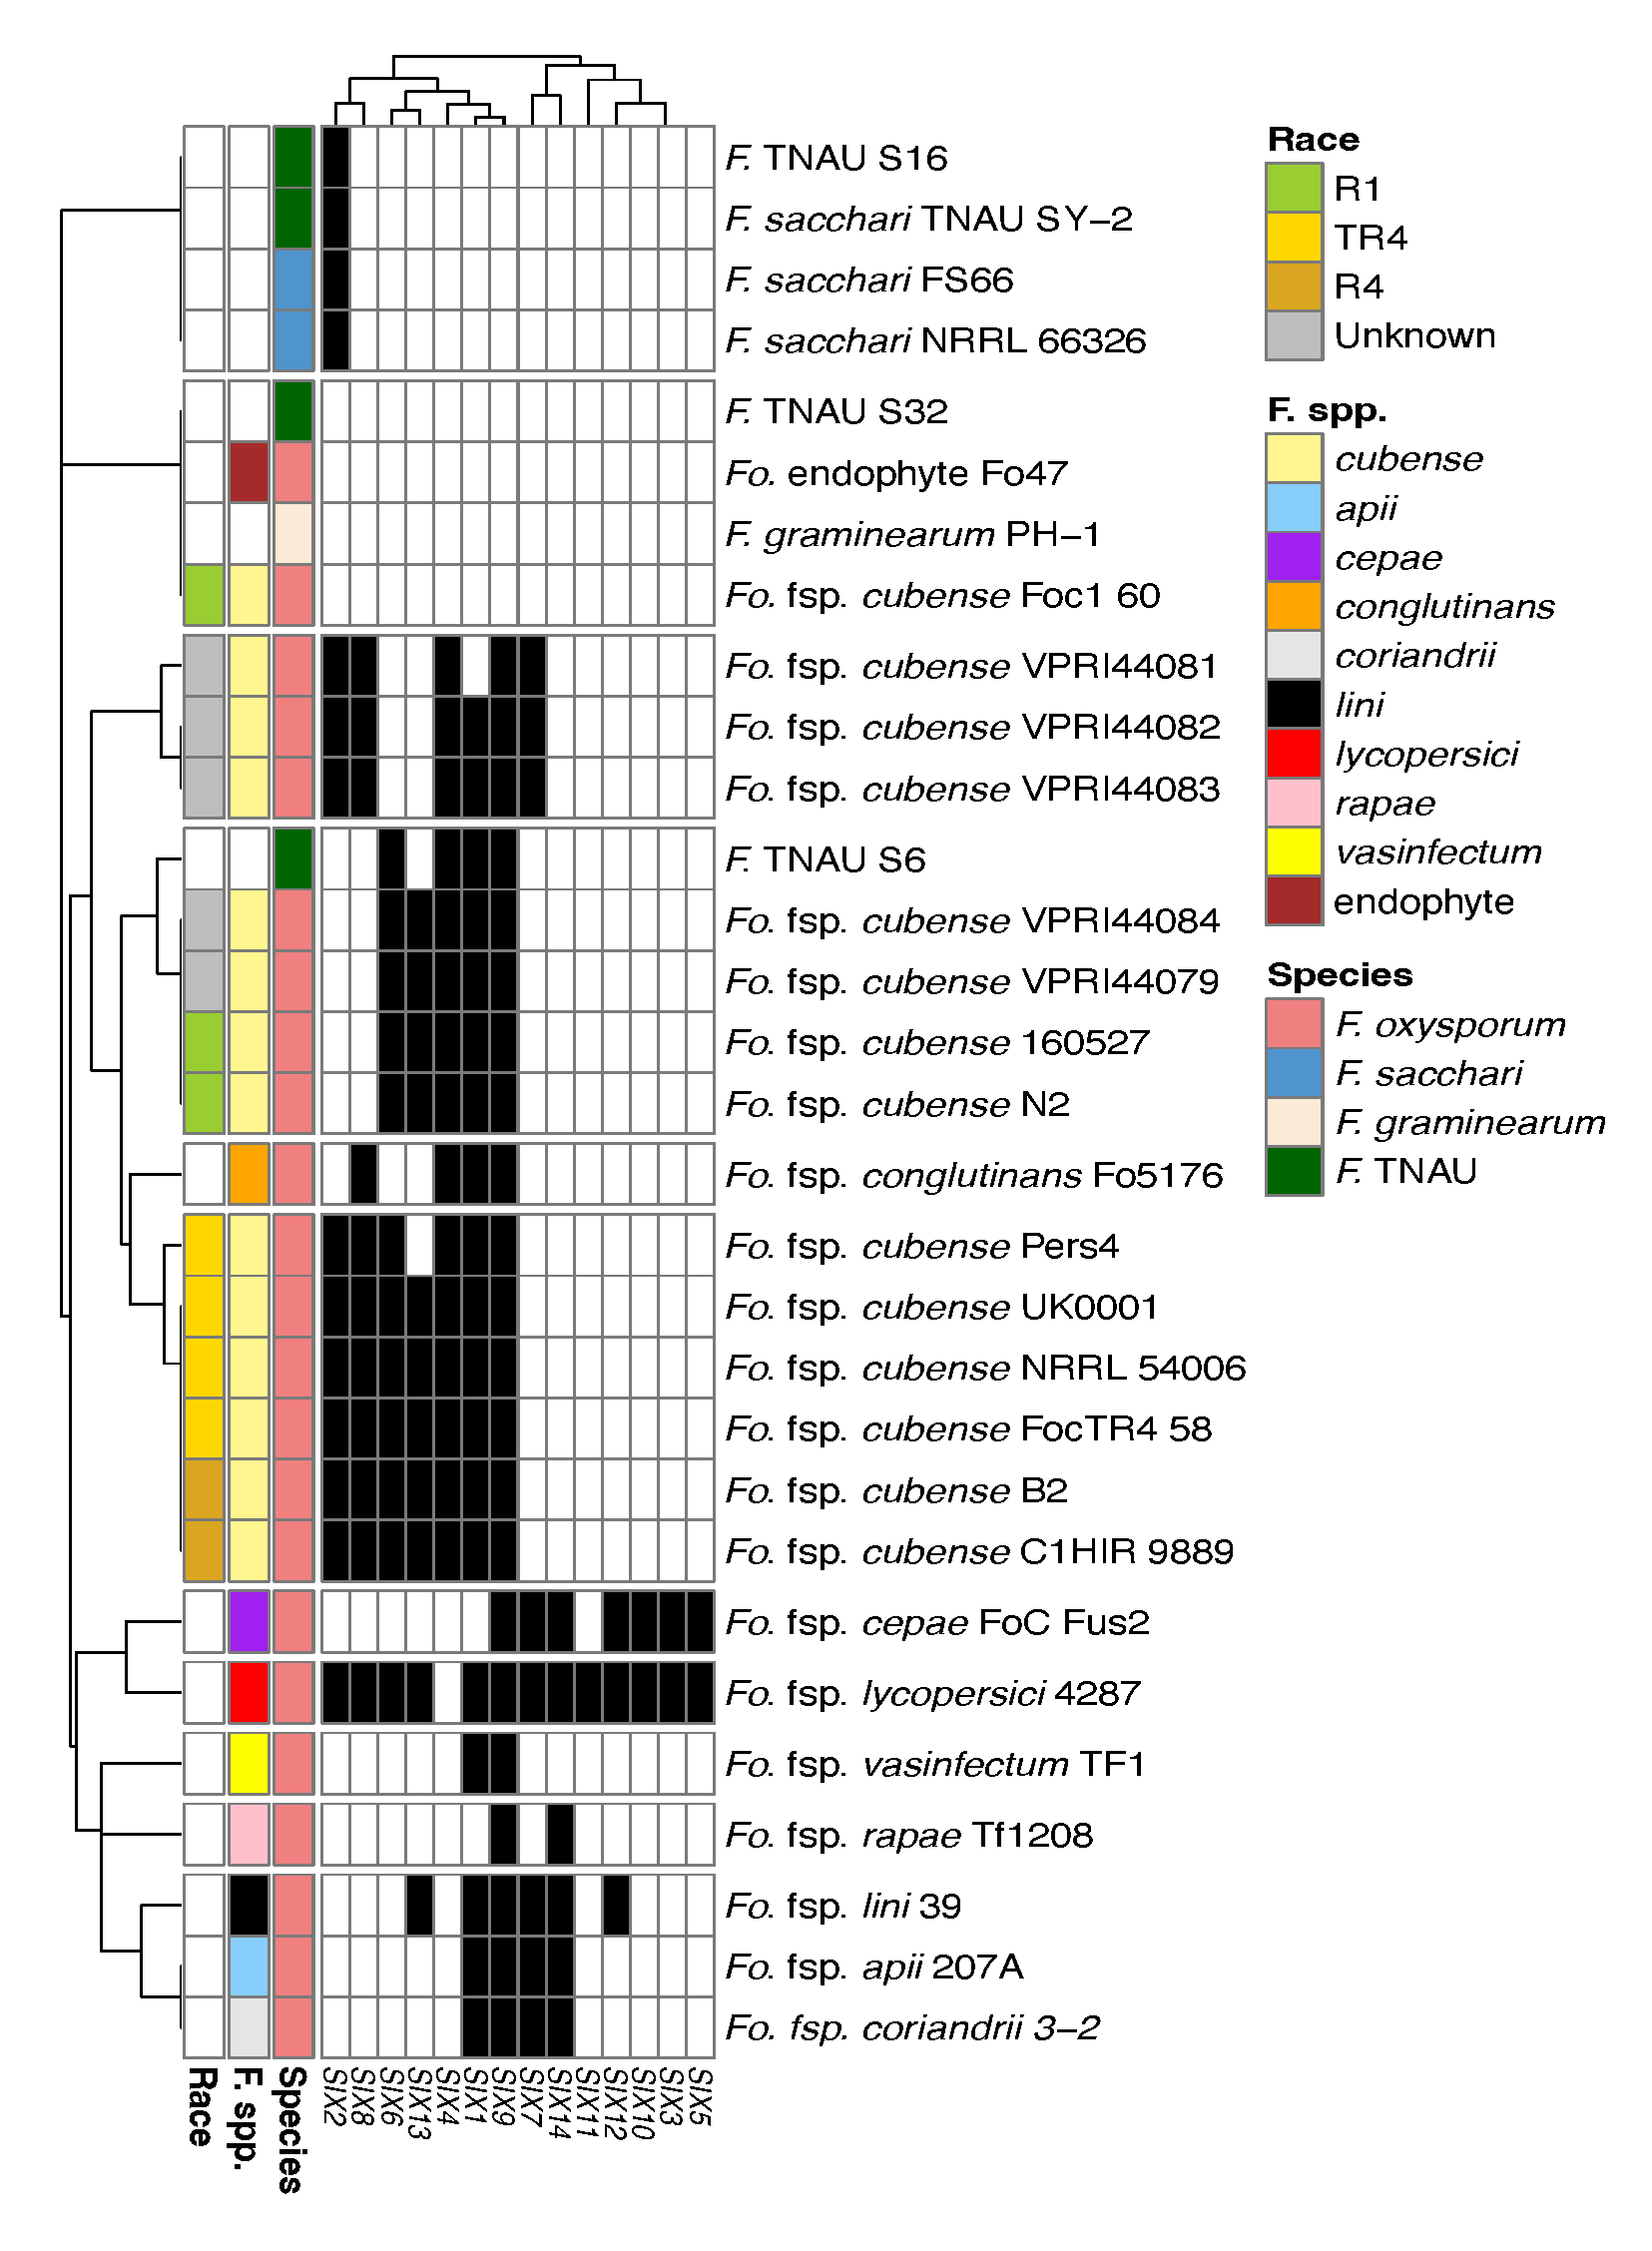
\includegraphics[width=15cm]{Figures/SixTNAU-Heatmap_edited.pdf}
  \caption[Binary distribution of \textit{SIX} genes across Fusarium TNUA isolates]{\textbf{Binary distribution of \textit{SIX} genes across Fusarium TNUA isolates}. \acl{sixg} identified using tBLASTn (cut off 1\-e\^6) using SIX genes from F. oxysporum fsp. lycopersici as a reference. \textit{SIX4} not found in the \ac{Fol} 4287 assembly, supported by previous publications e.g. Czislowski et al., 2017.}
  \label{fig:SixTNAU}
\end{figure}
\bigskip

\bigskip
\begin{figure}[htp!]
  \centering
  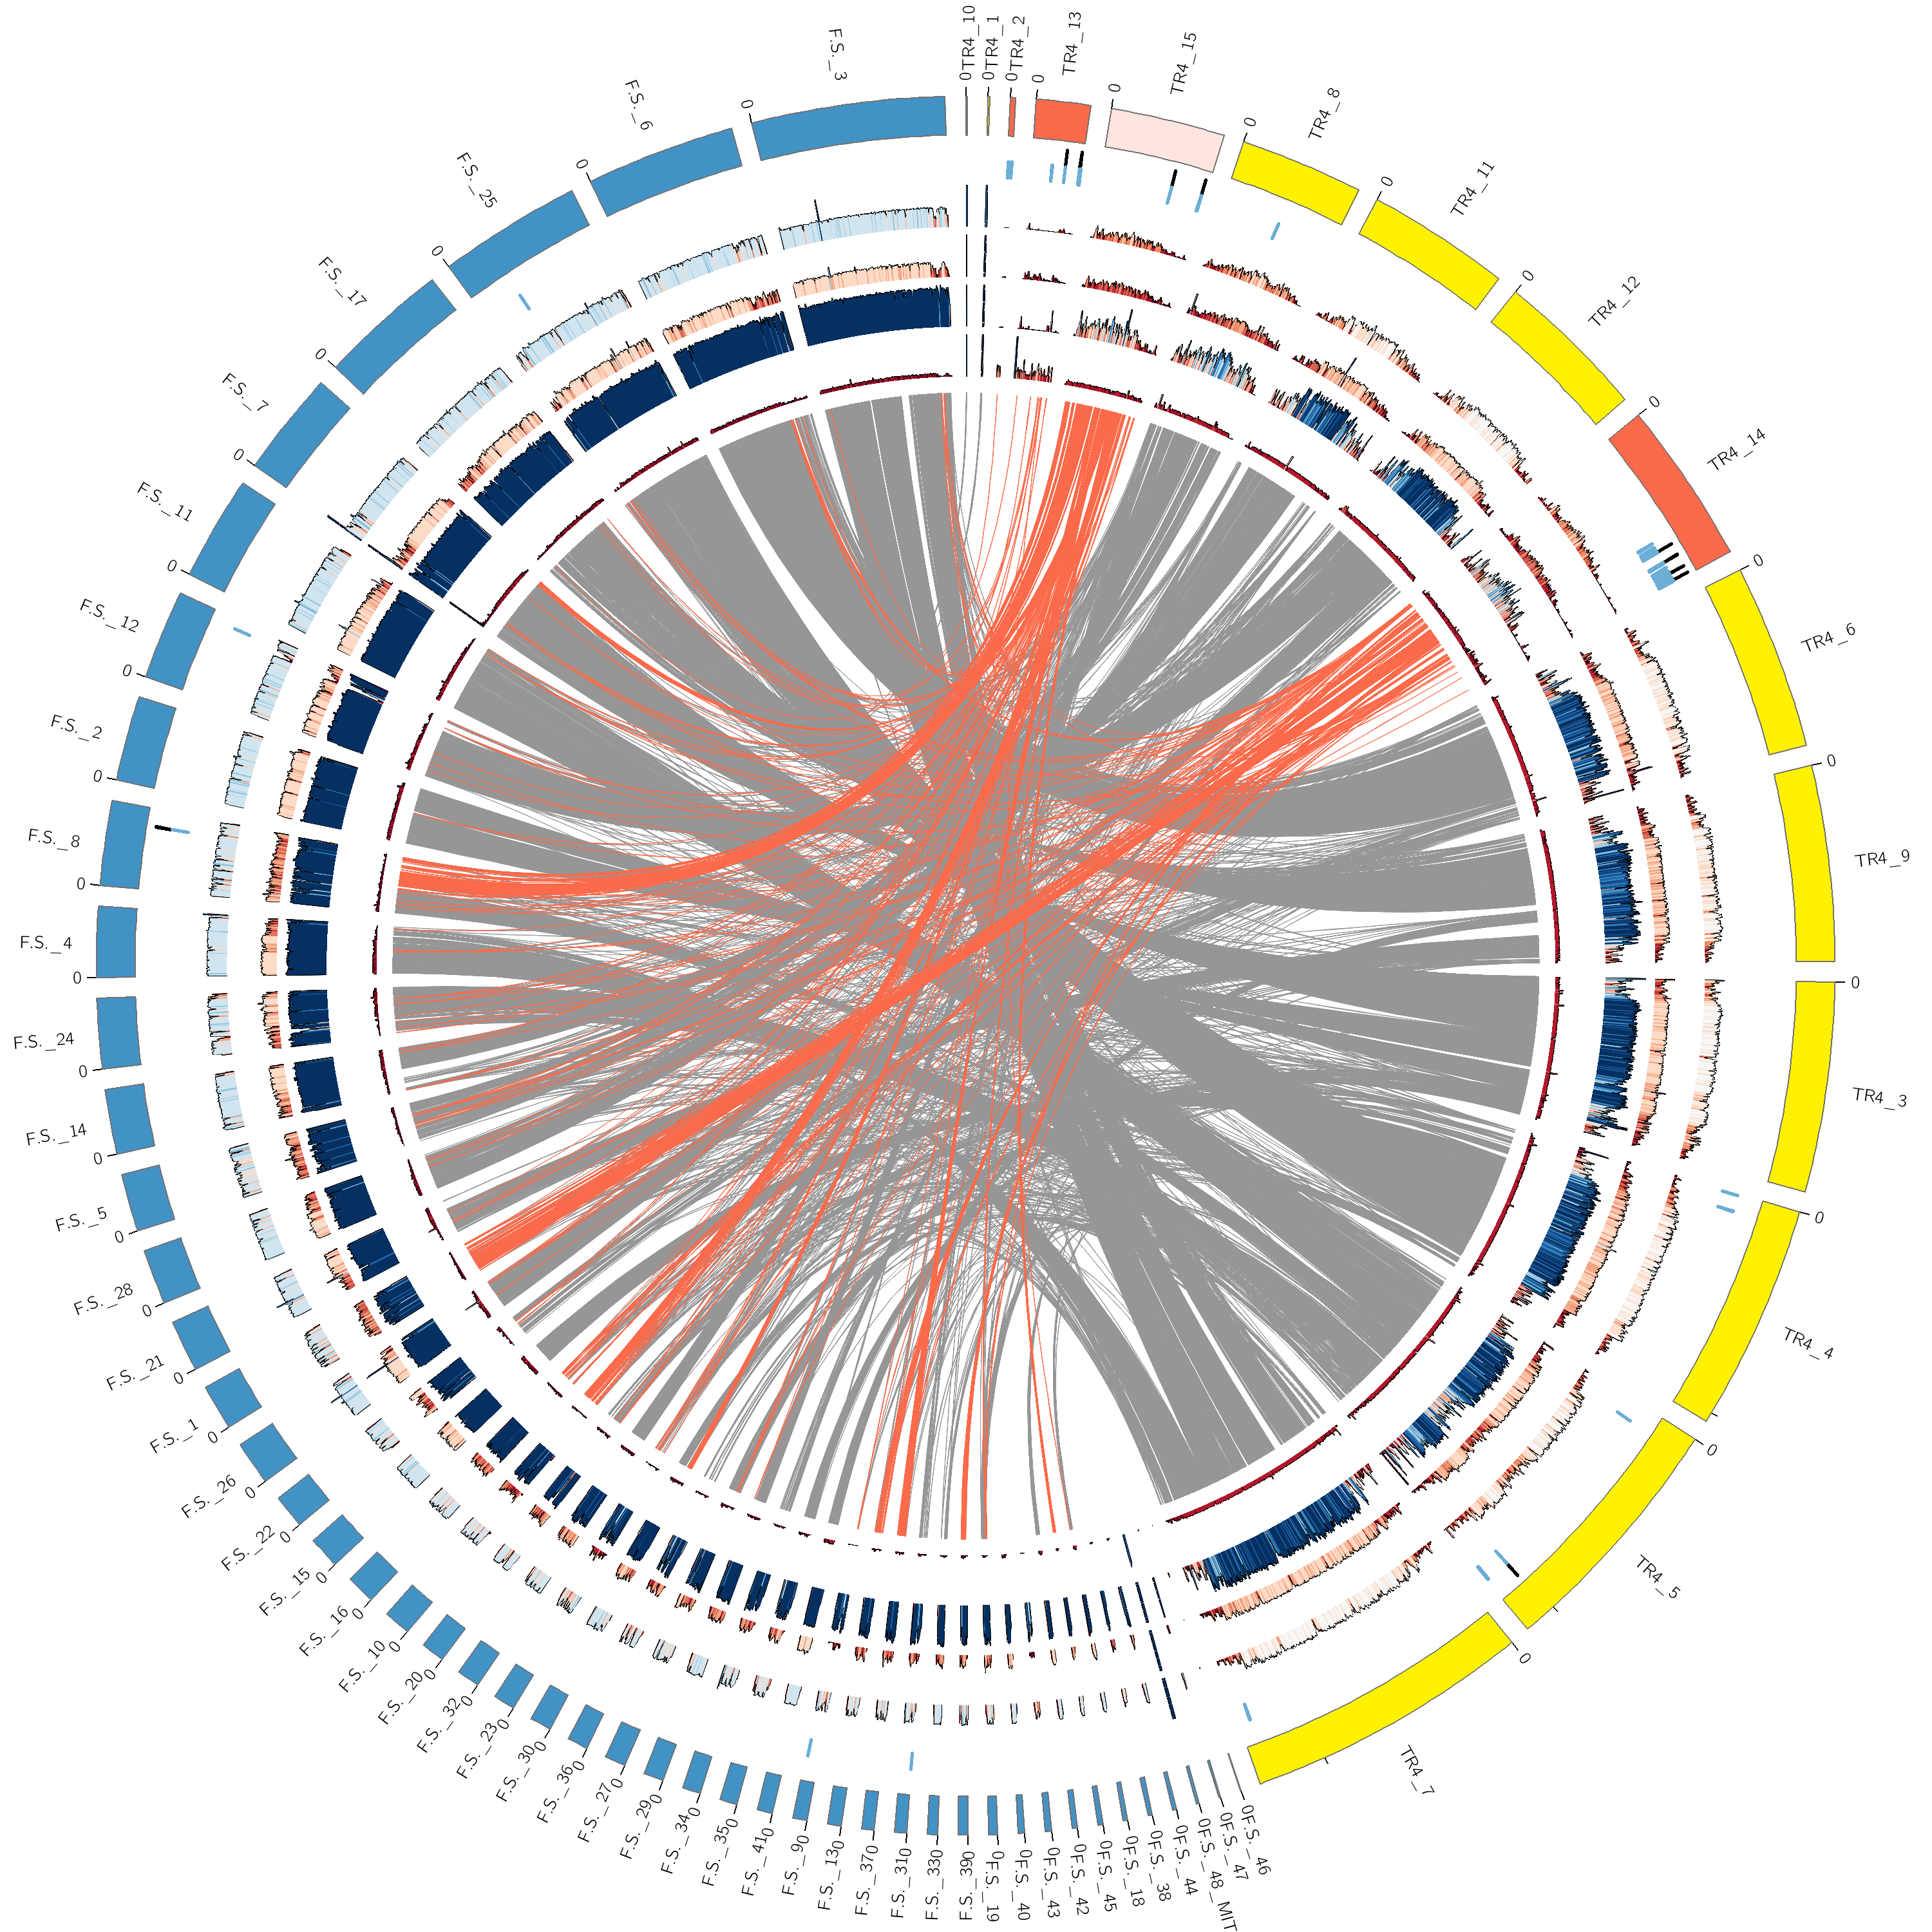
\includegraphics[width=15cm]{Figures/circos.png}
  \caption[Circos Plot of FS66 vs UK0001, including mapping data form TNAU isolates]{\textbf{Circos Plot of FS66 vs UK0001, including mapping data form TNAU isolates}}
  \label{TNAUCircos}
\end{figure}
\bigskip

\subsubsection{EffectorP and MIMPS Searching outputs. Any effectors which have homology to Foc predicted effectors?}


%%%%%%%%%%%%%%%%%%%%%%%%%%%%%%%%%%%%%%%%%%%%%
%DISCUSSION
%%%%%%%%%%%%%%%%%%%%%%%%%%%%%%%%%%%%%%%%%%%%%
\newpage
\section{Discussion and Conclusions}
\subsection{Strength of genotyping and phenotyping – why does genotyping say it is Foc?}
\subsection{\textit{De novo} Genome Assembly and Contamination Analysis}

Using the raw reads that appear to be contaminated to generate a \textit{de novo} assembly may result in misassembled contigs that are chimeric (part target species, part non-target species). These contigs can be challenging to identify and may result in contigs that should remain in the assembly being filtered out, and contigs that do not belong to the target species being kept in the assembly, even when using BlobTools to separate target and non-target contigs. A reference-guided assembly approach was considered, however, as isolates S16 and S32 have a higher mapping rate to the \textit{F. saccahri} reference and assemblies generated using all raw reads contained contigs that shared greater sequence similarity with other \textit{Fusarium} species, but these isolates have been classified as \textit{F. oxysporum} f. sp. \textit{cubense} isolates by collaborators at TNAU, determining which reference species to use is challenging. Furthermore, these isolates display a highly virulent phenotype, and a reference-guided assembly may lose any large-scale rearrangements in the genome which may play a role in this. Consequently, isolates S6 and S32, were assembled using the reads which mapped to reference genomes with the highest mapping value. For S6, therefore, a \textit{de novo} assembly was generated using the raw reads which mapped to \ac{Focub1} 160527 (\href{https://www.ncbi.nlm.nih.gov/datasets/genome/GCA_005930515.1/}{GCA\_005930515.1}) reference and for S32 a \textit{de novo} assembly was generated using the raw reads which mapped to
the \textit{Fusairum sacchari} FS66 (\href{https://www.ncbi.nlm.nih.gov/datasets/genome/GCA_017165645.1/}{GCA\_017165645.1}) reference.  

\subsubsection{High level of contamination from Stenotrophomonas.}
\subsection{Downstream analysis and quality of interpretation?}
- data not great but taken together suggest nov. sp. 
\subsection{Newly emerging banana pathogen -link to intro}
New banana path appearing at place where largest banana prod is. 

also this tho... https://apsjournals.apsnet.org/doi/10.1094/PDIS-09-20-2052-PDN 
\subsubsection{Similar results from Philippines paper.}

